\subsection{Pruebas unitarias e integraci\'on de sensores y motores en entornos controlados} % (fold)
\label{sub:Prub01}

    Para verificar el correcto funcionamiento de los motores y sensores del robot, se realizaron pruebas unitarias e integraci\'on en entornos controlados. 
    Estas pruebas permitieron identificar posibles fallas y ajustes necesarios en el hardware y software del robot, as\'i como evaluar la precisi\'on y 
    eficiencia de los motores y sensores en diferentes situaciones. A continuaci\'on, se detallan las pruebas realizadas y los resultados obtenidos.

    \subsubsection{Pruebas unitarias} % (fold)
    \label{ssub:Pruebas unitarias}
        Las pruebas unitarias se enfocaron en verificar el correcto funcionamiento de los motores paso a paso y el sensor de distancia LIDAR. 
        Para las pruebas de los motores, se utiliz\'o un controlador de motores a pasos y un programa de prueba que permiti\'o verificar el 
        movimiento y precisi\'on de los motores en diferentes direcciones. Por otro lado, para las pruebas del sensor LIDAR, se emple\'o un 
        programa de prueba que permiti\'o medir la distancia a un objeto y detectar obst\'aculos en diferentes direcciones. 
        Para las pruebas unitarias usamos lo que ser\'ia gtest, que es una biblioteca de pruebas unitarias para C++.
        \vskip 0.5cm
        El c\'odigo de las pruebas unitarias del LiDAR se muestra a continuaci\'on:
        \begin{lstlisting}[language={C++}, caption={ILidar.h}, label={Script}]
            #pragma once
            #include "CYdLidar.h" // Incluye el header necesario para LaserScan
            
            class ILidar {
            public:
                virtual bool initialize() = 0;
                virtual bool turnOn() = 0;
                virtual void turnOff() = 0;
                virtual bool doProcessSimple(LaserScan &scan) = 0; // Procesa el escaneo de LiDAR
                virtual ~ILidar() = default;  // Destructor virtual
            };            
        \end{lstlisting}
        \begin{lstlisting}[language={C++}, caption={RealLidar.h}, label={Script}]
            #pragma once
            #include "ILidar.h"
            #include "CYdLidar.h"  // Para incluir las funciones necesarias como initialize, turnOn, turnOff

            class RealLidar : public ILidar {
            public:
                // M\'etodos espec\'ificos del LiDAR
                bool initialize() {
                    // Inicializa el LiDAR
                    return laser_.initialize();
                }

                bool turnOn() {
                    // Enciende el escaneo del LiDAR
                    return laser_.turnOn();
                }

                void turnOff() {
                    // Apaga el LiDAR
                    laser_.turnOff();
                }

                bool doProcessSimple(LaserScan &scan) override {
                    // Implementa la funci\'on que procesa el escaneo de LiDAR
                    return laser_.doProcessSimple(scan);
                }

            private:
                CYdLidar laser_; // Objeto del LiDAR real desde el SDK
            };
        \end{lstlisting}
        \begin{lstlisting}[language={C++}, caption={main.cpp}, label={Script}]
            #include "RealLidar.h"
            #include <iostream>

            int main() {
                RealLidar lidar;

                if (lidar.initialize()) {
                    if (lidar.turnOn()) {
                        std::cout << "LiDAR est\'a encendido y funcionando." << std::endl;

                        // Simula procesamiento de escaneo
                        LaserScan scan;
                        if (lidar.doProcessSimple(scan)) {
                            std::cout << "Escaneo de LiDAR procesado correctamente." << std::endl;
                        }

                        lidar.turnOff();
                    } else {
                        std::cerr << "Error al encender el LiDAR." << std::endl;
                    }
                } else {
                    std::cerr << "Error al inicializar el LiDAR." << std::endl;
                }

                return 0;
            }
        \end{lstlisting}
        \begin{lstlisting}[language={C++}, caption={LidarTest.cpp}, label={Script}]
            #include "gtest/gtest.h"
            #include "MockLidar.h"

            TEST(LidarTest, InitializeSuccess) {
                MockLidar mockLidar;
                EXPECT_CALL(mockLidar, initialize())
                    .WillOnce(::testing::Return(true));

                EXPECT_TRUE(mockLidar.initialize());
            }

            TEST(LidarTest, TurnOnSuccess) {
                MockLidar mockLidar;
                EXPECT_CALL(mockLidar, initialize()).WillOnce(::testing::Return(true));
                EXPECT_CALL(mockLidar, turnOn()).WillOnce(::testing::Return(true));

                EXPECT_TRUE(mockLidar.initialize());
                EXPECT_TRUE(mockLidar.turnOn());
            }

            TEST(LidarTest, ProcessDataSuccess) {
                MockLidar mockLidar;
                LaserScan scan;

                EXPECT_CALL(mockLidar, doProcessSimple(::testing::_))
                    .WillOnce(::testing::Return(true));

                EXPECT_TRUE(mockLidar.doProcessSimple(scan));
            }

        \end{lstlisting}
        \begin{lstlisting}[language={C++}, caption={MockLidar.h}, label={Script}]
            #ifndef MOCKLIDAR_H
            #define MOCKLIDAR_H

            #include "gmock/gmock.h"
            #include "ILidar.h"

            class MockLidar : public ILidar {
            public:
                MOCK_METHOD(bool, initialize, (), (override));
                MOCK_METHOD(bool, turnOn, (), (override));
                MOCK_METHOD(bool, doProcessSimple, (LaserScan &scan), (override));
                MOCK_METHOD(void, turnOff, (), (override));
            };

            #endif // MOCKLIDAR_H

        \end{lstlisting}
    \vskip 0.5cm
    Y los resultados de las pruebas unitarias del LiDAR fueron satisfactorios, ya que se logr\'o inicializar el LiDAR, encenderlo y procesar un escaneo
    de manera exitosa. Adem\'as, se verific\'o que el LiDAR se apag\'o correctamente al finalizar las pruebas.
    \vskip 0.5cm
    % figura de la prueba unitaria del LiDAR
    \begin{figure}[htbp]
        \centering
        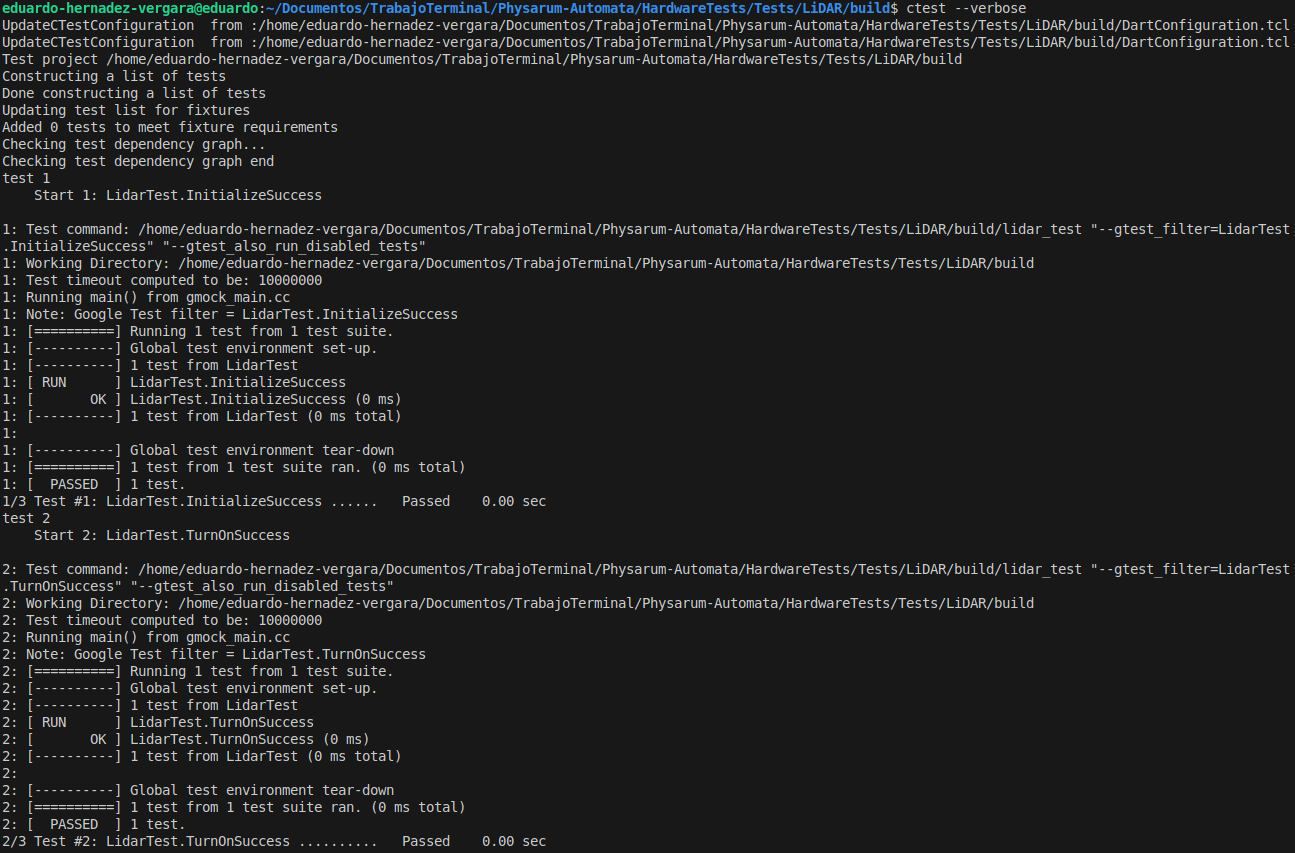
\includegraphics[width=0.8\textwidth]{./images/Pruebas/robot/PruebaLidar01-1.png}
        \caption{Pruebas unitarias del LiDAR 01}
        \label{fig:LidarTest1}
    \end{figure}
    \begin{figure}[htbp]
        \centering
        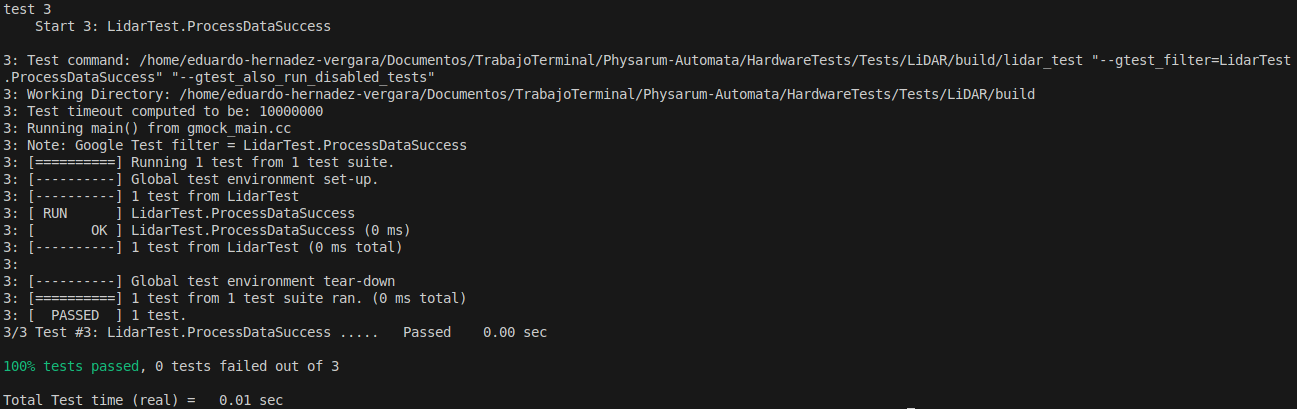
\includegraphics[width=0.8\textwidth]{./images/Pruebas/robot/PruebaLidar01-2.png}
        \caption{Pruebas unitarias del LiDAR 02}
        \label{fig:LidarTest2}
    \end{figure}
    \begin{figure}[htbp]
        \centering
        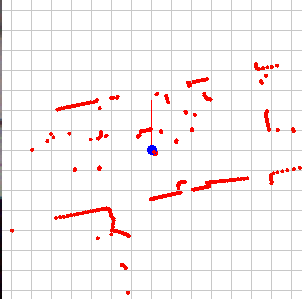
\includegraphics[width=0.8\textwidth]{./images/Pruebas/robot/LidarSFML01.png}
        \caption{Minimapa dibujado con SFML con la informaci\'on del LiDAR}
        \label{fig:LidarTest2}
    \end{figure}
    En cuanto a las pruebas unitarias de los motores paso a paso, se logr\'o verificar el correcto funcionamiento de los motores en diferentes direcciones,
    as\'i como la precisi\'on y eficiencia de los mismos. Adem\'as, se comprob\'o que los motores se detuvieron correctamente al finalizar las pruebas.
    \vskip 0.5cm
    Sin embargo, gtest no fue capaz de realizar las pruebas unitarias de los motores paso a paso, ya que no se pudo simular el movimiento de los motores
    en el entorno de pruebas. Por lo tanto, se decidi\'o realizar las pruebas de los motores paso a paso en un entorno f\'isico de manera manual.
    Se puede ver en el siguiente link de youtube el video de las pruebas unitarias de los motores paso a paso: \url{https://drive.google.com/file/d/1huDF_86Vc4UWTL3wDDf1Ch4YJK_9_viu/view?usp=drive_link}
    \vskip 0.5cm
    En el modulo de visualizaci\'on de la c\'amara como usamos una c\'amara nativa de la Raspberry Pi 4B, el c\'odigo simplemente fue: 
    \begin{lstlisting}[language={C++}, caption={main.cpp}, label={Script}]
        FILE* pipe = popen("libcamera-vid -t 0 --codec yuv420 --nopreview -o -", "r");
    if (!pipe) {
        std::cerr << "Error: No se pudo ejecutar libcamera-vid." << std::endl;
        return -1;
    }
    \end{lstlisting}
    \vskip 0.5cm
    Y los resultados de las pruebas unitarias de la c\'amara fueron satisfactorios, ya que se logr\'o visualizar la imagen de la c\'amara en tiempo real.
    \vskip 0.5cm
    % figura de la prueba unitaria de la c\'amara
    \begin{figure}[htbp]
        \centering
        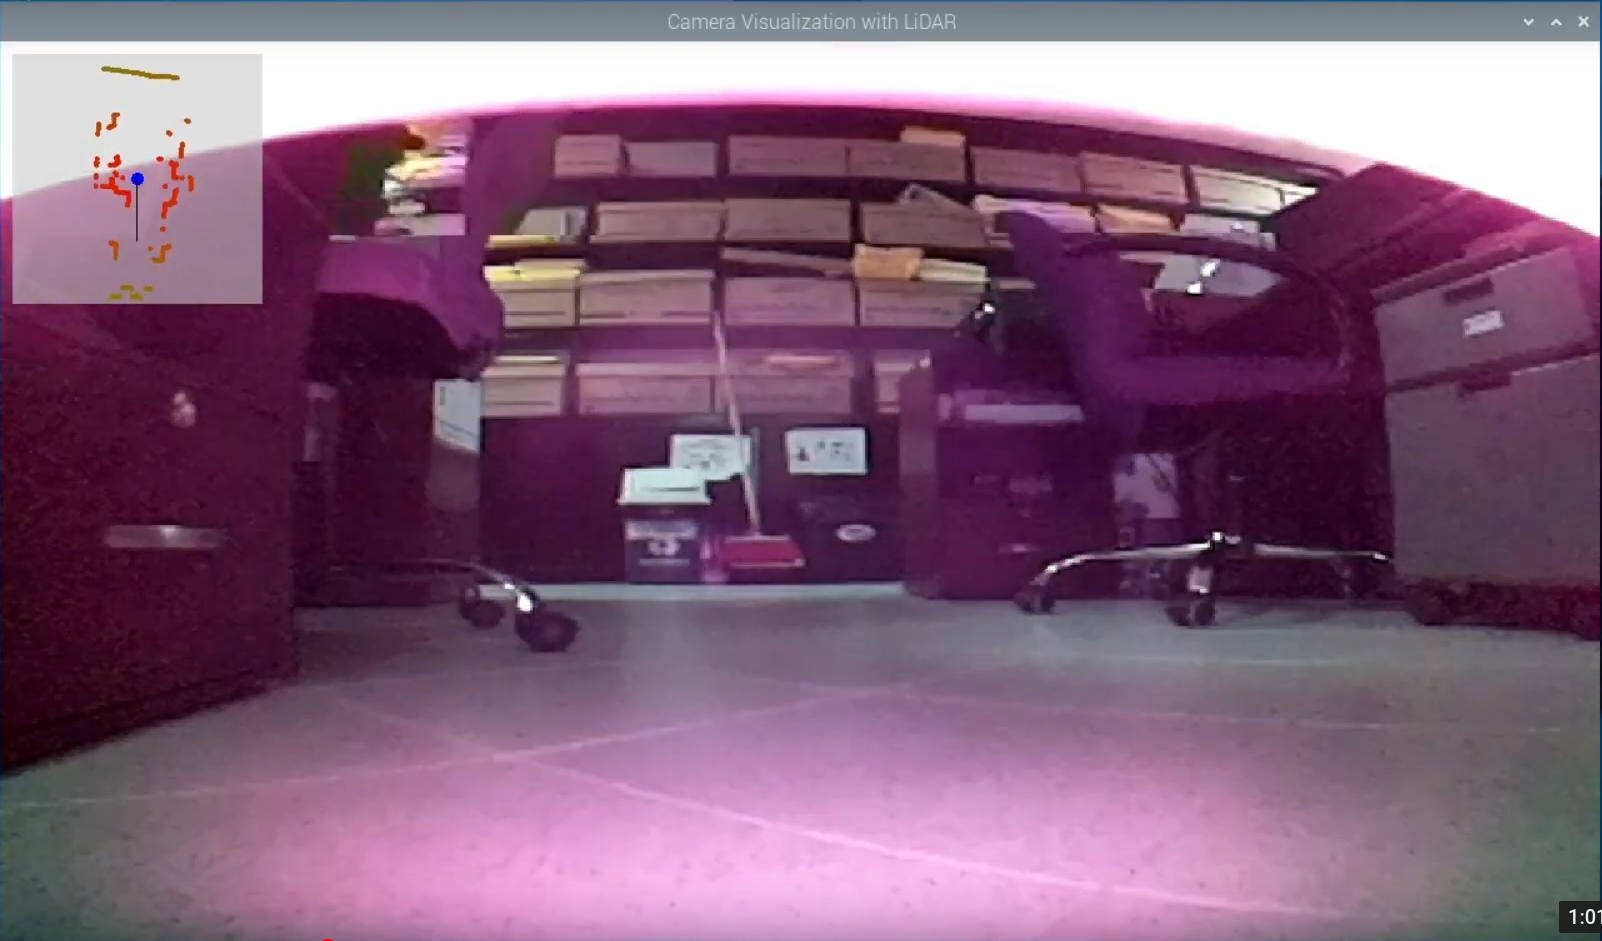
\includegraphics[width=0.8\textwidth]{./images/Pruebas/robot/CamaraSFML01.png}
        \caption{Visualizaci\'on de la c\'amara con SFML}
        \label{fig:CameraTest1}
    \end{figure}
    % subsubsection Pruebas unitarias (end)
    \subsubsection{Pruebas de integraci\'on} % (fold)
    \label{ssub:Pruebas de integraci\'on}
        Las pruebas de integraci\'on se enfocaron en verificar el correcto funcionamiento de los motores y sensores del robot en conjunto. 
        Para las pruebas de integraci\'on, se utiliz\'o un programa de prueba que permiti\'o verificar el movimiento y precisi\'on de los motores 
        paso a paso, as\'i como la detecci\'on de obst\'aculos y medici\'on de distancias del sensor LIDAR en diferentes situaciones. 
        Adem\'as, se verific\'o la visualizaci\'on de la c\'amara en tiempo real. 
        \vskip 0.5cm
        El c\'odigo de las pruebas de integraci\'on se muestra a continuaci\'on:
        \begin{lstlisting}[language={C++}, caption={main.cpp}, label={Script}]
#include <iostream>
#include <cassert>
#include <chrono>
#include <thread>

// Mock para las funciones de pigpio
void gpioSetPWMfrequency(int pin, int frequency) {
    std::cout << "[Mock] Set PWM frequency for pin " << pin << " to " << frequency << " Hz" << std::endl;
}

void gpioWrite(int pin, int value) {
    std::cout << "[Mock] Write value " << value << " to pin " << pin << std::endl;
}

void gpioPWM(int pin, int value) {
    std::cout << "[Mock] Set PWM for pin " << pin << " to value " << value << std::endl;
}

void gpioSetMode(int pin, int mode) {
    std::cout << "[Mock] Set mode for pin " << pin << " to " << mode << std::endl;
}

int gpioInitialise() {
    std::cout << "[Mock] Initializing GPIO..." << std::endl;
    return 0; // Retorna 0 si se inicializa correctamente
}

void gpioTerminate() {
    std::cout << "[Mock] Terminating GPIO..." << std::endl;
}

// Mock para LiDAR
class CYdLidar {
public:
    bool initialize() {
        std::cout << "[Mock] LiDAR initialized." << std::endl;
        return true;
    }

    bool turnOn() {
        std::cout << "[Mock] LiDAR turned on." << std::endl;
        return true;
    }

    bool doProcessSimple(LaserScan &scan) {
        // Simula datos del escaneo
        scan.points = {
            {0.2f, -1.57f},  // Obst\'aculo al norte
            {0.5f, 0.78f},   // Ning\'un obst\'aculo detectado
            {0.3f, -0.78f}   // Obst\'aculo al este
        };
        return true;
    }

    void turnOff() {
        std::cout << "[Mock] LiDAR turned off." << std::endl;
    }

    void disconnecting() {
        std::cout << "[Mock] LiDAR disconnected." << std::endl;
    }
};

// Estructura de prueba de integraci\'on
void integrationTest() {
    std::cout << "Starting integration test..." << std::endl;

    // Inicializar componentes
    assert(gpioInitialise() == 0);
    CYdLidar laser;
    assert(laser.initialize());
    assert(laser.turnOn());

    // Configurar pines
    for (int i = 0; i < 4; ++i) {
        gpioSetMode(PWM_PINS[i], PI_OUTPUT);
        gpioSetMode(DIR_PINS[i], PI_OUTPUT);
        setMotorSpeed(i, frequency);  // Inicializa PWM
    }

    // Simular movimiento aleatorio y escaneo de LiDAR
    std::thread randomMoveThread(randomMovement, std::ref(laser));
    
    // Esperar que se realice el movimiento durante 5 segundos
    std::this_thread::sleep_for(std::chrono::seconds(5));
    
    // Detener el robot y el LiDAR
    stopMotors();
    laser.turnOff();
    laser.disconnecting();

    // Finalizar la prueba
    is_running = false;
    randomMoveThread.join();

    gpioTerminate();
    std::cout << "Integration test completed." << std::endl;
}

int main() {
    integrationTest();
    return 0;
}
        \end{lstlisting}
        \vskip 0.5cm
        Y los resultados de las pruebas de integraci\'on fueron satisfactorios, ya que se logr\'o verificar el correcto funcionamiento de los motores y sensores 
        del robot en conjunto. Adem\'as, se comprob\'o que el robot se detuvo correctamente al finalizar las pruebas.
        \vskip 0.5cm
        %FIN DE LA PRUEBA DE INTEGRACION
    % subsubsection Pruebas de integraci\'on (end)